%\documentclass[handout]{beamer} 
\documentclass[t,12pt,numbers,fleqn]{beamer}
%\documentclass[ignorenonframetext]{beamer}

\newif\ifquestions
%\questionstrue
\questionsfalse

\usepackage{pgfpages} 
\usepackage{hyperref}
\hypersetup{colorlinks=true,
    linkcolor=blue,
    citecolor=blue,
    filecolor=blue,
    urlcolor=blue,
    unicode=false}
\urlstyle{same}

\usepackage{booktabs}
\usepackage{hhline}
\usepackage{multirow}
\usepackage{multicol}
\usepackage{array}

\bibliographystyle{plainnat}

%\usetheme{Iimenau}

\useoutertheme{split} %so the footline can be seen, without needing pgfpages

%\pgfpagesuselayout{resize to}[letterpaper,border shrink=5mm,landscape]  %if this is uncommented, the hyperref links do not work

\mode<presentation>{}

%% Requires:
%% 
%% \usepackage{latexsym}
%% \usepackage{amssymb}
%% \usepackage{stmaryrd}

%\renewcommand{\labelenumi}{(\theenumi)}

\newcommand{\be}{\begin{enumerate}}
\newcommand{\ee}{\end{enumerate}}
\newcommand{\bi}{\begin{itemize}}
\newcommand{\ei}{\end{itemize}}
\newcommand{\bc}{\begin{center}}
\newcommand{\ec}{\end{center}}
\newcommand{\bsp}{\begin{sloppypar}}
\newcommand{\esp}{\end{sloppypar}}

\newcommand{\sglsp}{\ }
\newcommand{\dblsp}{\ \ }

\newcommand{\iclicker}{i\texttt{>}clicker}

\newcommand{\sA}{\mbox{$\cal A$}}
\newcommand{\sB}{\mbox{$\cal B$}}
\newcommand{\sC}{\mbox{$\cal C$}}
\newcommand{\sD}{\mbox{$\cal D$}}
\newcommand{\sE}{\mbox{$\cal E$}}
\newcommand{\sF}{\mbox{$\cal F$}}
\newcommand{\sG}{\mbox{$\cal G$}}
\newcommand{\sH}{\mbox{$\cal H$}}
\newcommand{\sI}{\mbox{$\cal I$}}
\newcommand{\sJ}{\mbox{$\cal J$}}
\newcommand{\sK}{\mbox{$\cal K$}}
\newcommand{\sL}{\mbox{$\cal L$}}
\newcommand{\sM}{\mbox{$\cal M$}}
\newcommand{\sN}{\mbox{$\cal N$}}
\newcommand{\sO}{\mbox{$\cal O$}}
\newcommand{\sP}{\mbox{$\cal P$}}
\newcommand{\sQ}{\mbox{$\cal Q$}}
\newcommand{\sR}{\mbox{$\cal R$}}
\newcommand{\sS}{\mbox{$\cal S$}}
\newcommand{\sT}{\mbox{$\cal T$}}
\newcommand{\sU}{\mbox{$\cal U$}}
\newcommand{\sV}{\mbox{$\cal V$}}
\newcommand{\sW}{\mbox{$\cal W$}}
\newcommand{\sX}{\mbox{$\cal X$}}
\newcommand{\sY}{\mbox{$\cal Y$}}
\newcommand{\sZ}{\mbox{$\cal Z$}}

\renewcommand{\phi}{\varphi}
\newcommand{\seq}[1]{{\langle #1 \rangle}}
\newcommand{\set}[1]{{\{ #1 \}}}
\newcommand{\tuple}[1]{{( #1 )}}
\newcommand{\mlist}[1]{{[ #1 ]}}
\newcommand{\sembrack}[1]{\llbracket#1\rrbracket}
%\newcommand{\sembrack}[1]{[\![#1]\!]}
\newcommand{\synbrack}[1]{\ulcorner#1\urcorner}
\newcommand{\commabrack}[1]{\lfloor#1\rfloor}
\newcommand{\bsynbrack}[1]{\lceil#1\rceil}
\newcommand{\bsembrack}[1]{\lceil\!\!\lceil#1\rceil\!\!\rceil}
\newcommand{\mname}[1]{\mbox{\sf #1}}
\newcommand{\mcolon}{\mathrel:}
\newcommand{\mdot}{\mathrel.}
\newcommand{\modpar}{\models_{\rm par}}
\newcommand{\modreg}{\models_{\rm reg}}
\newcommand{\proves}[2]{#1 \vdash #2}
\newcommand{\notproves}[2]{#1 \not\vdash #2}
\newcommand{\provesin}[3]{#1 \vdash_{#2} #3}
\newcommand{\notprovesin}[3]{#1 \not\vdash_{#2} #3}
%\newcommand{\leqq}[1]{\mathrel{\preceq_{#1}}}
\newcommand{\parrow}{\rightharpoonup}
\newcommand{\tarrow}{\rightarrow}
\newcommand{\term}{\seq}
\newcommand{\lub}{\sqcup}
\newcommand{\subfun}{\sqsubseteq}
\newcommand{\subpred}{\subseteq}
\newcommand{\BoxApp}{\Box\,}
\newcommand{\BOX}{\mathrel{\Box}}
\newcommand{\funapp}{\mathrel@}

\newcommand{\com}{\mname{complement}}
\newcommand{\dom}{\mname{domain}}
\newcommand{\sumcl}{\mname{sum}}
\newcommand{\pow}{\mname{power}}
\newcommand{\pair}{\mname{pair}}
\newcommand{\opair}{\mname{ordered-pair}}
\newcommand{\inters}{\mname{intersection}}
\newcommand{\emp}{\mname{empty}}
\newcommand{\uni}{\mname{univocal}}
\newcommand{\fun}{\mname{function}}
\newcommand{\card}{\mname{card}}
\newcommand{\sets}{\mname{sets}}
\newcommand{\monotone}{\mname{monotone}}
\newcommand{\continuous}{\mname{continuous}}
\newcommand{\chain}{\mname{chain}}
\newcommand{\mub}{\mname{ub}}
\newcommand{\mlub}{\mname{lub}}
\newcommand{\fixedpoint}{\mname{fp}}
\newcommand{\leastfixedpoint}{\mname{lfp}}
\newcommand{\strongfixedpoint}{\mname{sfp}}
\newcommand{\emptyfun}{\triangle}
\newcommand{\statetrans}[1]{\stackrel{#1}{\longrightarrow}}
\newcommand{\thyext}{\leq}
\newcommand{\conthyext}{\unlhd}

\newcommand{\Iota}{\mbox{\rm I}}
\newcommand{\IotaApp}{\mbox{\rm I}\,}
\newcommand{\iotaApp}{\iota\,}
\newcommand{\epsilonApp}{\epsilon\,}
\newcommand{\True}{\mbox{\sf T}} 
\newcommand{\False}{\mbox{\sf F}} 
\newcommand{\Trueword}{\sf true}
\newcommand{\Falseword}{\sf false}
\newcommand{\Neg}{\neg} 
\newcommand{\Andd}{\wedge}
\newcommand{\Or}{\vee}
\newcommand{\Implies}{\supset}
\newcommand{\ImpliesAlt}{\Rightarrow}
\newcommand{\Iff}{\equiv}
\newcommand{\Sheffer}{\mathrel|}
\newcommand{\IffAlt}{\Leftrightarrow}
\newcommand{\Forall}{\forall}
\newcommand{\ForallApp}{\forall\,}
\newcommand{\Forsome}{\exists}
\newcommand{\ForsomeApp}{\exists\,}
\newcommand{\ForsomeUniqueApp}{\exists\,!\,}
\newcommand{\IsDef}{\downarrow}
\newcommand{\IsUndef}{\uparrow}
\newcommand{\Equal}{=}
\newcommand{\QuasiEqual}{\simeq}
\newcommand{\Undefined}{\bot}
\newcommand{\If}{\mname{if}}
\newcommand{\IsDefApp}{\!\IsDef}
\newcommand{\IsUndefApp}{\!\IsUndef}
\newcommand{\TRUE}{\mbox{{\sc t}}}
\newcommand{\FALSE}{\mbox{{\sc f}}}
\newcommand{\truthvalues}{\{\TRUE,\FALSE\}}
\newcommand{\LambdaApp}{\lambda\,}
\newcommand{\LAMBDAapp}{\Lambda\,}
\newcommand{\AlphaEquiv}{\stackrel{\alpha}{=}}

\newcommand{\mvar}[3]{\textbf{var}_{#1}[#2,#3]}
\newcommand{\mterm}[2]{\textbf{term}_{#1}[#2]}
\newcommand{\mform}[2]{\textbf{form}_{#1}[#2]}
\newcommand{\mtype}[2]{\textbf{type}_{#1}[#2]}
\newcommand{\mexpr}[3]{\textbf{expr}_{#1}[#2,#3]}

\newcommand{\imps}{\mbox{\sc imps}}
\newcommand{\fol}{\mbox{\sc fol}}
\newcommand{\lutins}{\mbox{\sc lutins}}
\newcommand{\vlisp}{\mbox{\sc vlisp}}
\newcommand{\vmach}{\mbox{\sc vmach}}
\newcommand{\gnu}{\mbox{\sc gnu}}
\newcommand{\zf}{\mbox{\sc zf}}
\newcommand{\nbg}{\mbox{\sc nbg}}
\newcommand{\pnbg}{\mbox{\sc pnbg}}
\newcommand{\snbg}{\mbox{\sc snbg}}
\newcommand{\pfol}{\mbox{\sc pfol}}
\newcommand{\nbgstar}{$\mbox{\sc nbg}^\ast$}
\newcommand{\boldnbgstar}{$\mbox{\bf NBG}^\ast$}
\newcommand{\stt}{\mbox{\sc stt}}
\newcommand{\eves}{\mbox{\sc eves}}
\newcommand{\hol}{\mbox{\sc hol}}
\newcommand{\mizar}{Mizar}
\newcommand{\nqthm}{Nqthm}
\newcommand{\pvs}{\mbox{\sc pvs}}
\newcommand{\stmm}{\mbox{\sc stmm}}

\iffalse
\newtheorem{thm}{Theorem}[section]
\newtheorem{cor}[thm]{Corollary}
\newtheorem{lem}[thm]{Lemma}
\newtheorem{prop}[thm]{Proposition}
\newtheorem{rem}[thm]{Remark}
\newtheorem{eg}[thm]{Example}
\newtheorem{df}[thm]{Definition}
\fi

%\newenvironment{proof}{\par\noindent{\bf Proof\ \ }}{$\Box$}

\newenvironment{namedform}[1]
   {\begin{tabbing}\textbf{#1}\ }
   {\end{tabbing}}

\newcommand{\urlpart}[1]{\mbox{\texttt{#1}}\linebreak[0]}

\newcommand{\bblue}{\textcolor{blue!80!black}}
\newcommand{\bgreen}{\textcolor{green!55!black}}
\newcommand{\bbrown}{\textcolor{brown}}
\newcommand{\bred}{\textcolor{red!80!black}}
\newcommand{\bcyan}{\textcolor{cyan!80!black}}
\newcommand{\bmagenta}{\textcolor{magenta}}
\newcommand{\byellow}{\textcolor{yellow}}
\newcommand{\borange}{\textcolor{orange}}
\newcommand{\bviolet}{\textcolor{violet}}
\newcommand{\bpurple}{\textcolor{purple}}
\newcommand{\bdarkgray}{\textcolor{darkgray}}
\newcommand{\bgray}{\textcolor{gray}}
\newcommand{\blightgray}{\textcolor{lightgray}}

\newcommand{\clicker}{i\texttt{>}clicker}

\newenvironment{changemargin}[2]{%
  \begin{list}{}{%
    \setlength{\topsep}{0pt}%
    \setlength{\leftmargin}{#1}%
    \setlength{\rightmargin}{#2}%
    \setlength{\listparindent}{\parindent}%
    \setlength{\itemindent}{\parindent}%
    \setlength{\parsep}{\parskip}%
  }%
  \item[]}{\end{list}}


\newcommand{\topic}{03 Requirements DRAFT}

%Title page information for 1D04 lectures slides

% Define year specific parameters - used in title page and footer

\newcommand{\season}{Fall} %use to switch between Winter and Fall
\newcommand{\instructor}{Dr.~Spencer Smith} %use to switch instructor
\newcommand{\instructSmall}{Dr.~Smith}
\newcommand{\yr}{2017}
\newcommand{\courseCode}{CAS 741, CES 741}
\newcommand{\courseTitle}{Development of Scientific Computing Software}

%\setbeamerfont{structure}{series=\bfseries}
%\usefonttheme[stillsansseriftext,stillsansserifmath]{serif}
\setbeamertemplate{navigation symbols}{} 
\setbeamertemplate{itemize item}[ball]

\title{
  {\normalsize \bf 
    \borange{\courseCode~(\courseTitle)\\ \season~\yr}}\\[2ex]
  {\Large \bf \topic}}

\author[Smith]{\instructor}

\institute{
  Faculty of Engineering,
  McMaster University}

\date{
\today
%January 2011\\
\bc
  
\includegraphics[scale = 0.2, keepaspectratio]
  {../mcmaster-logo-full-color.jpg}
\ec
}

\renewcommand{\borange}[1] %orange is too hard to read
{
   \bred{#1}
}

\begin{document}

% Footline for  Slides

% Display title page and displays footers

\setbeamertemplate{footline}{} %so the title screen does not have a footline

%%%%%%%%%%%%%%%%%%%%%%%%%%%%%%%%%%%%%%%%%%%%%%%%%%%%%%%%%%%%

\begin{frame}
\titlepage
\end{frame}

%%%%%%%%%%%%%%%%%%%%%%%%%%%%%%%%%%%%%%%%%%%%%%%%%%%%%%

\setbeamertemplate{footline}{
\begin{beamercolorbox}{sectioninhead/foot}
\hspace{1ex}\bblue{\hrulefill}\hspace{1ex}

\vspace{1ex}
\hspace{1ex}
{\tiny \instructSmall \hfill 
\courseCode~\season~\yr:~\topic \hfill 
\insertframenumber/\inserttotalframenumber~~}
%\insertframenumber/\ref{lastframe}}
%\hfill {\small \insertframenumber} \hspace{10ex}
%{\small $$\insertframenumber$$}
\vspace{1ex}
\end{beamercolorbox}}

%%%%%%%%%%%%%%%%%%%%%%%%%%%%%%%%%%%%%%%%%%%%%%%%%%%%%%


%%%%%%%%%%%%%%%%%%%%%%%%%%%%%%%%%%%%%%%%%%%%%%%%%%%%%%

\begin{frame}
\frametitle{Requirements}

\bi
\item Administrative details
\item Questions: project choices, software tools
\item License and copyright
\item Motivation
\begin{itemize}
\item Scientific Computing Software Qualities
\item Challenges to Developing Quality Scientific Software
\end{itemize}
\item Requirements documentation for scientific computing
\item A new requirements template
\item Advantages of new template and examples
\item The new template from a software engineering perspective
\item Concluding remarks
\item References
\ei
\end{frame}

%%%%%%%%%%%%%%%%%%%%%%%%%%%%%%%%%%%%%%%%%%%%%%%%%%%%%%

\begin{frame}
\frametitle{Administrative Details}

\bi
\item Add me to your GitHub repos, my GitHub id is \texttt{smiths}
\ei

\end{frame}

%%%%%%%%%%%%%%%%%%%%%%%%%%%%%%%%%%%%%%%%%%%%%%%%%%%%%%

\begin{frame}
\frametitle{Administrative Details: Report Deadlines}
~\newline
\begin{tabular}{l l l}
\textbf{Problem Statement} & Week 02 & Sept 15\\
System Requirements Specification (SRS) & Week 05 & Oct 4\\
Verification and Validation Plan & Week 07 & Oct 25\\
Module Guide (MG) & Week 09 & Nov 8\\
Module Interface Specification (MIS) & Week 11 & Nov 22\\
Final Documentation & Week 13 & Dec 6\\
\end {tabular}

\bi
\item The written deliverables will be graded based on the repo contents as of
11:59 pm of the due date
\item If you need an extension, please ask
\item Two days after each major deliverable, your GitHub issues will be due
\ei

\end{frame}

%%%%%%%%%%%%%%%%%%%%%%%%%%%%%%%%%%%%%%%%%%%%%%%%%%%%%%

\begin{frame}
\frametitle{Administrative Details: Presentations}

~\newline
\begin{tabular}{l l l}
SRS Present & Week 04 & Week of Sept 25\\
V\&V Present & Week 06 & Week of Oct 16\\
MG Present & Week 08 & Week of Oct 30\\
MIS Present & Week 10 & Week of Nov 13\\
Implementation Present & Week 12 & Week of Nov 27\\
\end {tabular}

\bi
\item Tentative dates
\item Specific schedule depends on final class registration and need
\item Informal presentations with the goal of improving everyone's written
  deliverables
\ei

\end{frame}

%%%%%%%%%%%%%%%%%%%%%%%%%%%%%%%%%%%%%%%%%%%%%%%%%%%%%%

\begin{frame}

\frametitle{Important Qualities for Scientific Computing Software}

\begin{itemize}

\item External qualities
\begin{itemize}
\item Correctness (Thou shalt not lie)
\item Reliability
\item Robustness
\item Performance
\begin{itemize}
%\item Tight bounds
\item Time efficiency
\item Space efficiency
\end{itemize}
\end{itemize}

\item Internal qualities
\begin{itemize}
\item Verifiability
%\item Productivity
\item Usability
\item Maintainability
%\begin{itemize}
%\item Repairability
%\item Evolvability
%\end{itemize}
\item Reusability
\item Portability
\end{itemize}

\end{itemize}

\end{frame}

%%%%%%%%%%%%%%%%%%%%%%%%%%%%%%%%%%%%%%%%%%%%%%%%%%%%%%

\begin{frame}

\frametitle{Problems with Developing Quality Scientific Computing Software}

\begin{itemize}

\item Need to know requirements to judge reliability
\item In many cases the only documentation is the code
\item Reuse is not as common as it could be
\begin{itemize}
\item \href{http://www.andrew.cmu.edu/user/sowen/softsurv.html}{\alert{Meshing software survey}}
\item \href{http://www.engr.usask.ca/~macphed/finite/fe_resources/node137.html}{\alert{Public domain finite element
programs}}
\item etc.
\end{itemize}
\item Many people develop ``from scratch''
\item Cannot easily reproduce the work of others
\item Neglect of simple software development technology~\cite{Wilson2006} 
% such as version control software

\end{itemize}

\end{frame}

%%%%%%%%%%%%%%%%%%%%%%%%%%%%%%%%%%%%%%%%%%%%%%%%%%%%%%

\begin{frame}

\frametitle{Adapt Software Engineering Methodologies}

\begin{itemize}

\item Software engineering improves and quantifies quality %purpose of software engineering
\item Successfully applied in other domains
\begin{itemize}
\item Business and information systems
\item Embedded real time systems
\end{itemize}
\item Systematic engineering process
\item Design through documentation
\item Use of mathematics
\item Reuse of components
\item Warranty rather than a disclaimer %goal of software engineering

\end{itemize}

\end{frame}

%%%%%%%%%%%%%%%%%%%%%%%%%%%%%%%%%%%%%%%%%%%%%%%%%%%%%%

\begin{frame}

\frametitle{Developing Scientific Computing Software}

\begin{itemize}

\item Facilitators
\begin{itemize}
\item One user viewpoint for specifying a physical model
\item Assumptions can be used to distinguish models
\item High potential for reuse
\item Libraries
\item Already mathematical
\end{itemize}

\item Challenges
\begin{itemize}
\item Verification and Validation
\item Acceptance of software engineering methodologies
\item No existing templates or examples %explain that templates are a tool for doc req.
\end{itemize}

\end{itemize}

\end{frame}

%%%%%%%%%%%%%%%%%%%%%%%%%%%%%%%%%%%%%%%%%%%%%%%%%%%%%%

\begin{frame}
\frametitle{Outline of Discussion of Requirements}

\begin{itemize}

\item Background on requirements elicitation, analysis and documentation
\item Tabular expressions
\item Why requirements analysis for engineering computation?

\item System Requirements Specification and template for beam analysis software
\begin{itemize}
\item Provides guidelines
\item Eases transition from general to specific
\item Catalyses early consideration of design
\item Reduces ambiguity
\item Identifies range of model applicability
\item Clear documentation of assumptions
\end{itemize}

\end{itemize}
\end{frame}

%%%%%%%%%%%%%%%%%%%%%%%%%%%%%%%%%%%%%%%%%%%%%%%%%%%%%%

\begin{frame}
\frametitle{A Rational Design Process}
%\begin{figure}
\begin{center}
 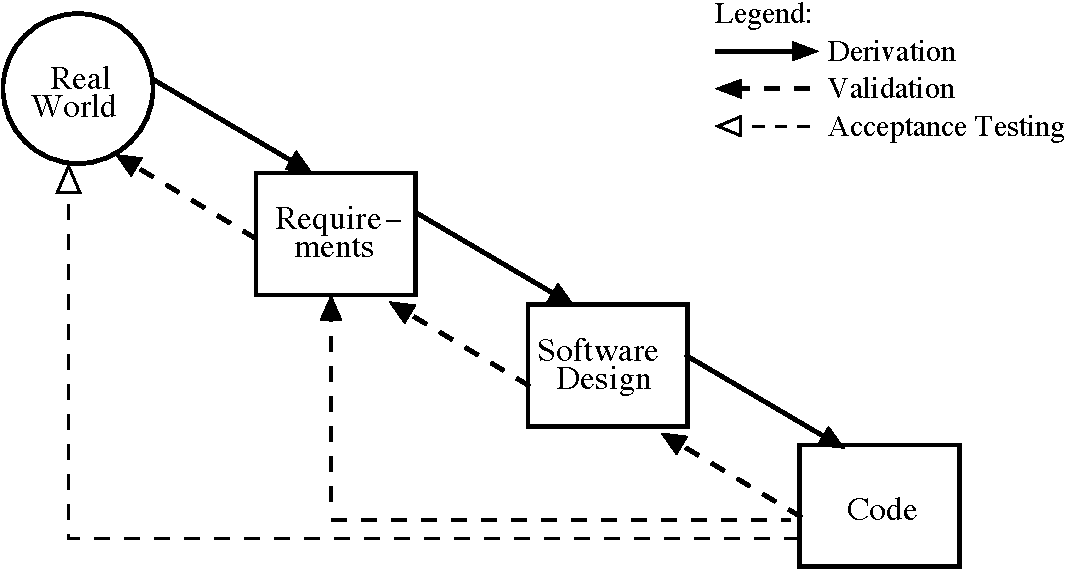
\includegraphics[width=1.0\textwidth]{../Figures/reqSE.pdf}
\end{center}
%\end{figure}
\end{frame}

%%%%%%%%%%%%%%%%%%%%%%%%%%%%%%%%%%%%%%%%%%%%%%%%%%%%%%

\begin{frame}
\frametitle{Sometimes Include Commonality Analysis}
%\begin{figure}
\begin{center}
 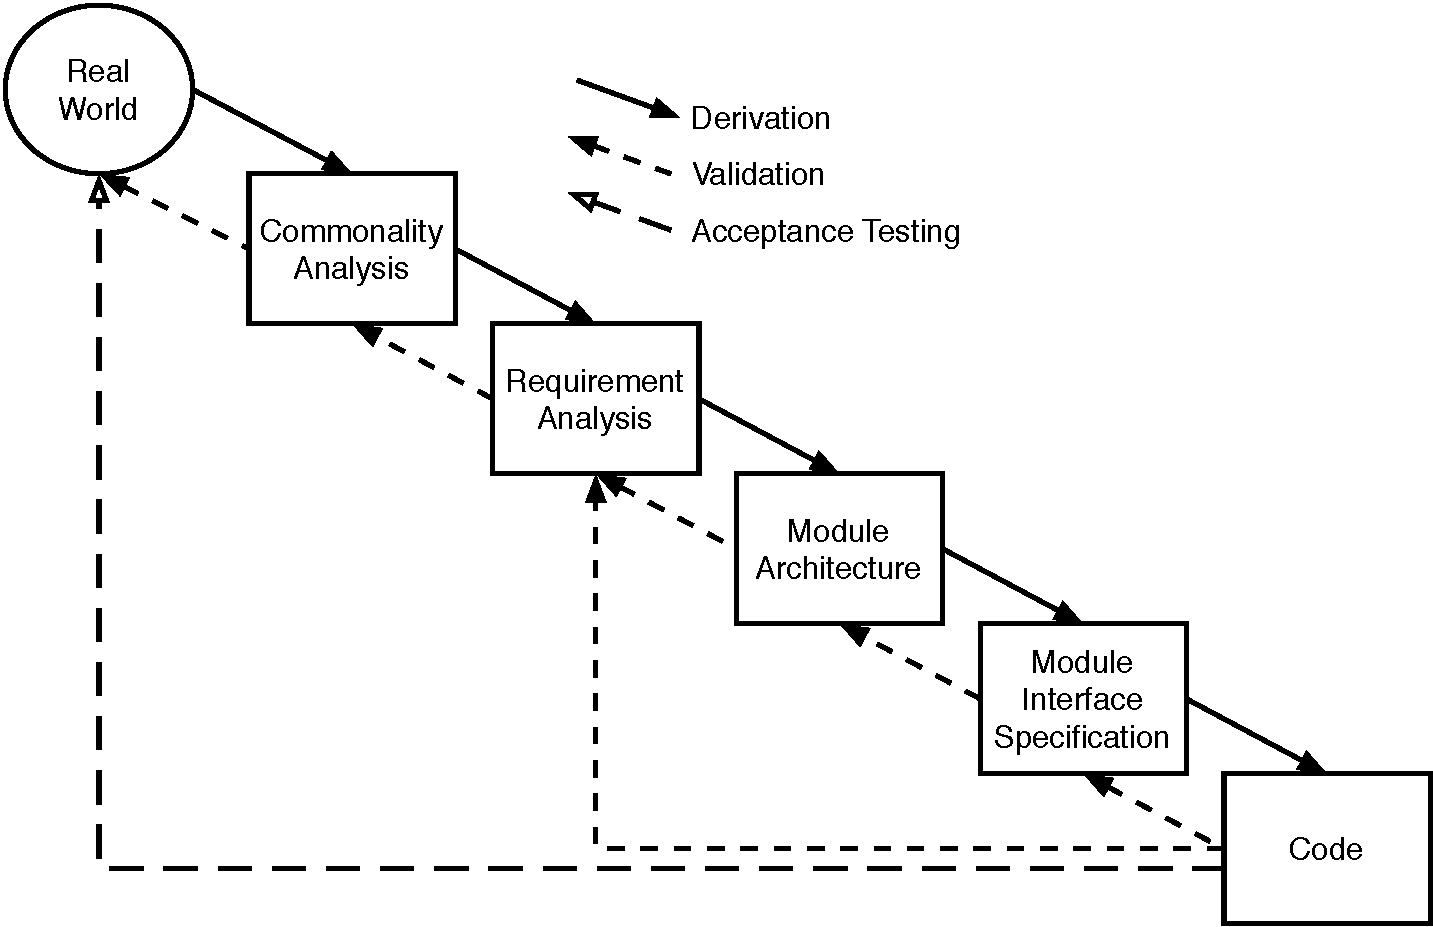
\includegraphics[width=1.0\textwidth]{../Figures/Waterfall.pdf}
\end{center}
%\end{figure}
\end{frame}

%%%%%%%%%%%%%%%%%%%%%%%%%%%%%%%%%%%%%%%%%%%%%%%%%%%%%%

\begin{frame}
\frametitle{Software Requirements Activities}
\begin{itemize}
\item A software requirement is a description of how the system should behave, or of a system property or attribute
\item Requirements should be unambiguous, complete, consistent, modifiable, verifiable and traceable
\item Requirements should express ``What'' not ``How''
\item Formal versus informal specification
\item Functional versus nonfunctional requirements
\item Software requirements specification (SRS)
\item Requirements template
\end{itemize}
\end{frame}

%%%%%%%%%%%%%%%%%%%%%%%%%%%%%%%%%%%%%%%%%%%%%%%%%%%%%%

\begin{frame}
\frametitle{Tabular Expressions}

\begin{flushleft}
\scalebox{0.75}{
\begin{tabular}{||r|p{6cm}||}
\hhline{=|=}
Composition rule & $\cup_{i=1}^{4} H_2[i] \cap  (\cap_{j=1}^{2} H_1[j] ~;~ G[i,j])$ \\
\hhline{=|=}
\end{tabular}
}
\end{flushleft}

%\begin{center}
\begin{tabular}{|l|p{0.3cm}|l|l|}
\multicolumn{4}{c}{} \\
\multicolumn{2}{c}{} & \multicolumn{2}{>{\large}c}{$H_1$} \\
\hhline{|~|~|-|-|}
\multicolumn{2}{c|}{} & $S_{GET}'\cup =$ & $ErrorMsg'+=$ \\
\hhline{|~|~|-|-|}
\multicolumn{4}{c}{} \\
\hhline{|-|~|-|-|}
$x_1 < 0$ & & $\emptyset$ & $InvalidInput\_x_1$  \\
\hhline{|-|~|-|-|}
$0 \le x_1 < min_d$ & & $\emptyset$ & $x_1\_TooSmall$ \\
\hhline{|-|~|-|-|}
$x_1 > max_d$ & & $\emptyset$ & $x_1\_TooLarge$ \\
\hhline{|-|~|-|-|}
$min_d \le x_1 \le max_d$ & & $\{@{x_1}\}$ & $NULL$ \\
\hhline{|-|~|-|-|}
\multicolumn{2}{c}{} & \multicolumn{2}{r}{$\land ChangeOnly(S_{GET}, ErrorMsg)$}\\
\multicolumn{2}{>{\large}c}{$H_2$} & \multicolumn{2}{>{\large}c}{$G$} \\
\end{tabular}
%\end{center}

\end{frame}

%%%%%%%%%%%%%%%%%%%%%%%%%%%%%%%%%%%%%%%%%%%%%%%%%%%%%%

\begin{frame}
\frametitle{Why Requirements Analysis?}
%\begin{figure}
\begin{center}
 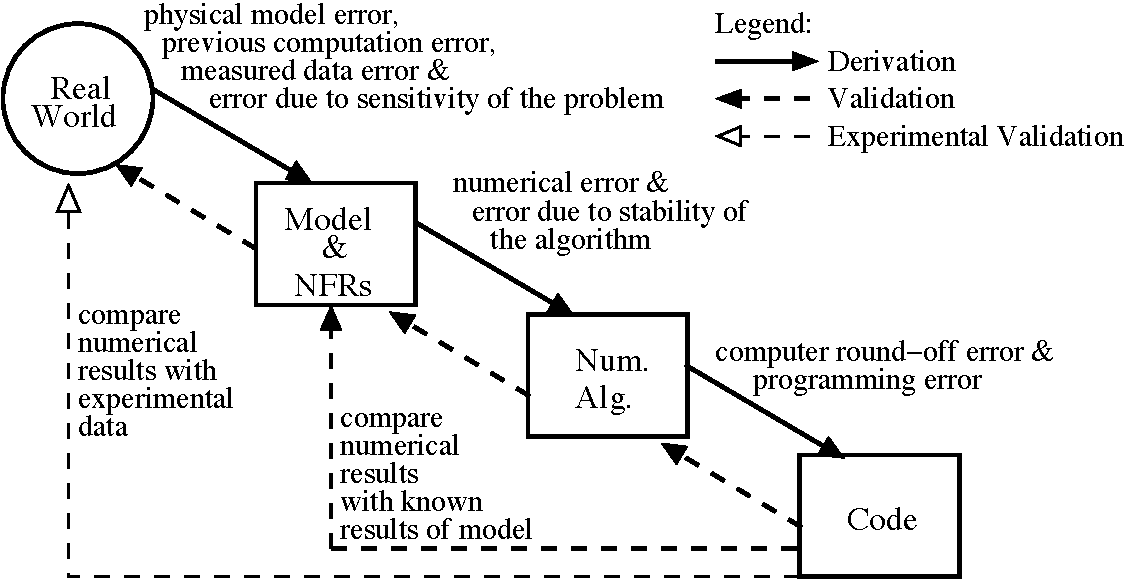
\includegraphics[width=1.0\textwidth]{../Figures/StagesInSciCompErrors.pdf}
\end{center}
%\end{figure}
\end{frame}

%%%%%%%%%%%%%%%%%%%%%%%%%%%%%%%%%%%%%%%%%%%%%%%%%%%%%%

\begin{frame}
\frametitle{Beam Analysis Software}
~\newline
~\newline
\begin{center}
 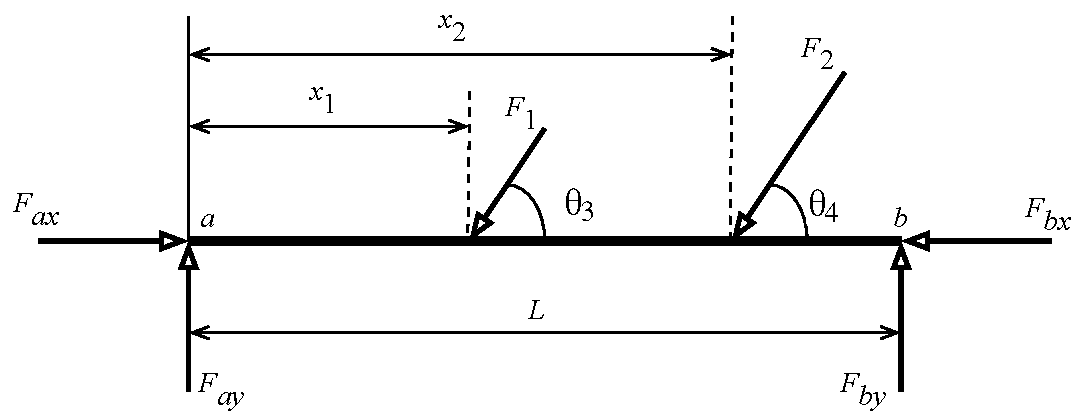
\includegraphics[width=1.0\textwidth]{../Figures/beamFBD.pdf}
\end{center}
\end{frame}

%%%%%%%%%%%%%%%%%%%%%%%%%%%%%%%%%%%%%%%%%%%%%%%%%%%%%%

\begin{frame}
\frametitle{Proposed Template}

\scalebox{0.85}{
\begin{minipage}{1.2\textwidth}
\begin{enumerate}

\item Reference Material: a) Table of Symbols ...

\item Introduction: a) Purpose of the Document; b) Scope of the Software Product; c) Organization of the Document.

\item General System Description: a) System Context; b) User Characteristics; c) System Constraints.

\item Specific System Description:
\begin{enumerate}
\item Problem Description: i) Background Overview ...
\item Solution specification: i) Assumptions; ii) Theoretical Models; ...
\item Non-functional Requirements: i) Accuracy of Input Data; ii) Sensitivity ...
\end{enumerate}

\item{Traceability Matrix}

\item List of Possible Changes in the Requirements

\item{Values of Auxiliary Constants}

\end{enumerate}
\end{minipage}
}
\end{frame}

%%%%%%%%%%%%%%%%%%%%%%%%%%%%%%%%%%%%%%%%%%%%%%%%%%%%%%

\begin{frame}
\frametitle{Provides Guidance}
\begin{itemize}
\item Details will not be overlooked, facilitates multidisciplinary collaboration
\item Encourages a systematic process
\item Acts as a checklist
\item Separation of concerns
\begin{itemize}
\item Discuss purpose separately from organization
\item Functional requirements separate from non-functional
%\begin{itemize}
%\item solve for forces
%\item system responds within 1 second
%\end{itemize}
\end{itemize}
\item Labels for cross-referencing
\begin{itemize}
\item Sections, physical system description, goal statements, assumptions, etc.
\item PS1.a ``the shape of the beam is long and thin''
\end{itemize}
%\item Use of parameters instead of explicit values
\end{itemize}
\end{frame}

%%%%%%%%%%%%%%%%%%%%%%%%%%%%%%%%%%%%%%%%%%%%%%%%%%%%%%

\begin{frame}
\frametitle{Eases Transition from General to Specific}
\begin{itemize}
\item ``Big picture'' first followed by details
\item Facilitates reuse
\item ``Introduction'' to ``General System Description'' to ``Specific System Description''
\item Refinement of abstract goals to theoretical model to instanced model
\begin{itemize}
\item \textbf{G1}. Solve for the unknown external forces applied to the beam
\item $ \textbf{T1}~ 
\textrm{$\sum{F_{xi}} = 0$,}~  
\textrm{$\sum{F_{yi}} = 0$,}~
\textrm{$\sum{M_i} = 0$}$
\item \textbf{M1} \textrm{$F_{ax} - F_1\cdot \cos\theta_3 - F_2\cdot \cos\theta_4 - F_{bx} = 0$}
\end{itemize}
\end{itemize}
\end{frame}

%%%%%%%%%%%%%%%%%%%%%%%%%%%%%%%%%%%%%%%%%%%%%%%%%%%%%%

\begin{frame}
\frametitle{Ensures Special Cases are Considered}
\scalebox{0.6}{
\begin{tabular}{| p{3.8cm} | p{1.7cm} | p{0.05cm} | p{9.0cm} | p{1.8cm} |}
\multicolumn{3}{c}{} & \multicolumn{2}{>{\large}c}{$H_1$} \\
\hhline{|~|~|~|-|-|}
\multicolumn{3}{c}{} & \multicolumn{1}{|c|}{$S_{GET} = S_{sym} - S_{unkF}$} & $S_{GET} \ne  (S_{sym} - S_{unkF})$ \\
\hhline{|~|~|~|-|-|}

\hhline{|-|-|~|-|-|} $S_{unkF} \notin \mathbb{P}_3$ & - &  & $(ErrorMsg'=InvalidUnknown)$ \newline
$\land ChangeOnly(ErrorMsg)$ &
\multirow{9}{2cm}{$FALSE$} \\
\hhline{|-|-|~|-|~|} $S_{unkF} = \newline \{@{F_{ax}}, @{F_{bx}}, @{F_{ay}} \}$ & - & & $ErrorMsg'=NoSolution$ \newline
$\land ChangeOnly(ErrorMsg)$ & \\
%\hhline{|-|-|~|-|~|} $S_{unkF} = \newline \{@{F_{ax}}, @{F_{bx}}, @{F_{by}} \}$ & - & & $ErrorMsg'=NoSolution$ \newline
%$\land ChangeOnly(ErrorMsg)$ & \\
%\hhline{|-|-|~|-|~|} $S_{unkF} = \newline \{@{F_{ax}}, @{F_{bx}}, @{F_1} \}$ & - & & $ErrorMsg'=NoSolution$ \newline
%$\land ChangeOnly(ErrorMsg)$ & \\
%\hhline{|-|-|~|-|~|} $S_{unkF} = \newline \{@{F_{ax}}, @{F_{bx}}, @{F_2} \}$ & - & & $ErrorMsg'=NoSolution$ \newline
%$\land ChangeOnly(ErrorMsg)$ & \\
\hhline{|-|-|~|-|~|}
%\multirow{3}{4.2cm}
{$S_{unkF} = \newline \{@{F_{ax}}, @{F_{ay}}, @{F_1}\}$} & 
$x_1 \ne 0 $ \newline
$\land~\theta_3 \ne 0$ \newline
$\land~\theta_3 \ne 180$
& & 
$F_{ax}' = $\newline
$\frac{-\cos\theta_3 F_2 x_2 \sin\theta_4 + \cos\theta_3 F_{by} L + F_2 \cos\theta_4 x_1 \sin\theta_3
+ F_{bx} x_1 \sin\theta_3}{x_1 \sin\theta_3}$\newline
$\land$\newline
$F_{ay}' = -\frac{F_2 x_2 \sin\theta_4 - F_{by} L - F_2 \sin\theta_4 x_1 + F_{by} x_1}{x_1}$\newline
{$\land~F_1' = \frac{-F_2 x_2 \sin\theta_4 + F_{by} L}{x_1 \sin\theta_3} \land ChangeOnly(S_{unkF})$}
& \\
\hhline{|~|-|~|-|~|} & $otherwise$ & & $(ErrorMsg'=Indeterminant)$\newline
$\land ChangeOnly(ErrorMsg)$ & \\
\hhline{|-|-|~|-|-|}

\multicolumn{5}{c}{} \\
\multicolumn{3}{>{\large}c}{$H_2$} & \multicolumn{2}{>{\large}c}{$G$} \\
\end{tabular} }
\end{frame}

%%%%%%%%%%%%%%%%%%%%%%%%%%%%%%%%%%%%%%%%%%%%%%%%%%%%%%

\begin{frame}
\frametitle{Catalyses Early Consideration of Design}
\begin{itemize}
\item Identification of significant issues early will improve the design
\item Section for considering sensitivity
\begin{itemize}
\item Conditioning?
\item Buckling of beam
\end{itemize}
\item Non-functional requirements
\begin{itemize}
\item Tradeoffs in design
\item Speed efficiency versus accuracy
\end{itemize}
\item Tolerance allowed for solution: $|\sum{F_{xi}}| / \sqrt{\sum{F_{xi}}^2} \le \epsilon$
\item Solution validation strategies
\item List of possible changes in requirements
\end{itemize}
\end{frame}

%%%%%%%%%%%%%%%%%%%%%%%%%%%%%%%%%%%%%%%%%%%%%%%%%%%%%%

\begin{frame}
\frametitle{Reduces Ambiguity}
\begin{itemize}
\item Unambiguous requirements allow communication between experts, requirements review, designers do not have to
make arbitrary decisions
\item Tabular expressions allow automatic verification of completeness
\item Table of symbols
\item Abbreviations and acronyms
\item Scope of software product and system context
\item User characteristics
\item Terminology definition and data definition
\item Ends arguments about the relative merits of different designs
\end{itemize}
\end{frame}

%%%%%%%%%%%%%%%%%%%%%%%%%%%%%%%%%%%%%%%%%%%%%%%%%%%%%%

\begin{frame}
\frametitle{Identifies Range of Model Applicability}
\begin{itemize}
\item Clear documentation as to when model applies
\item Can make the design specific to the problem
\item Input data constraints are identified
\begin{itemize}
\item Physically meaningful: $0 \leq x_1 \leq L$
\item Maintain physical description: PS1.a, $0 < h \leq 0.1 L$
\item Reasonable requirements: $0 \leq \theta_3 \leq 180$
\end{itemize}
\item The constraints for each variable are documented by tables, which are later composed together
\item $(min_f \le |F_{ax}| \le max_f) 
\land (|F_{ax}| \ne 0) \Rightarrow \forall ({FF}|{@{FF} \in S_F} \cdot {FF \ne 0
\land  \frac{max\{{|F_{ax}|,|FF|}\}}{min\{{|F_{ax}|, |FF|}\}} \le 10 ^ {r_f}})$
\end{itemize}
\end{frame}

%%%%%%%%%%%%%%%%%%%%%%%%%%%%%%%%%%%%%%%%%%%%%%%%%%%%%%
\begin{frame}

\frametitle{Summary of Variables}

\begin{table}
\begin{center}
\scalebox{0.9}{
\begin{tabular}{|l|l|p{3.0cm}|p{3.3cm}|l|}
\multicolumn{5}{c}{} \\
\hline
\textbf{Var} & \textbf{Type} & \textbf{Physical\newline Constraints} & \textbf{System\newline Constraints} &
\textbf{Prop} \\
\hline $x$ & $Real$ & $x\ge 0 \land x\le L$ & $min_d \le x \le max_d$ & NIV \\
\hline $x_1$ & $Real$ & $x_1\ge0 \land x_1\le L$ & $min_d \le x_1 \le max_d$ & IN \\
\hline $x_2$ & $Real$ & $x_2\ge0 \land x_2\le L$ & $min_d \le x_2 \le max_d$ & IN \\
\hline $e$ & $Real$ & $e>0 \land e \le h$ & $min_e \le e \le max_e$ & IN \\
\hline $h$ & $Real$ & $h>0 \land h\le 0.1L$ & $min_h \le h \le max_h$ & IN \\
\hline $L$ & $Real$ & $L>0$ & $min_d \le L \le max_d$ & IN \\
\hline $E$ & $Real$ & $E>0$ & $min_E \le E \le max_E$ & IN \\
\hline $\theta_3$ & $Real$ & $-\infty < \theta_3 < +\infty$ & $0 \le \theta_3 \le 180$ & IN \\
\hline $\theta_4$ & $Real$ & $-\infty < \theta_4 < +\infty$ & $0 \le \theta_4 \le 180$ & IN \\
\hline $V$ & $Real$ & $-\infty < V < +\infty$ & - & OUT \\
\hline $M$ & $Real$ & $-\infty < M < +\infty$ & - & OUT \\
\hline $y$ & $Real$ & $-\infty < y < +\infty$ & - & OUT \\
\hline $...$ & $...$ & $...$ & ... & ... \\
\hline
\end{tabular} }
\end{center}
\end{table}

\end{frame}

%%%%%%%%%%%%%%%%%%%%%%%%%%%%%%%%%%%%%%%%%%%%%%%%%%%%%%

\begin{frame}
\frametitle{Clear Documentation of Assumptions}
\scalebox{0.82}{
\begin{tabular}{| p{1.3cm} | p{1.3cm} | l | l | l | l | l | l | l | l | l | l | l | l |}
\hhline{--------------}
Phy. Sys. /Goal & Data /Model & \multicolumn{10}{c|}{Assumption} & \multicolumn{2}{c|}{Model} \\
\hhline{~~------------}
&  & A1 & A2 & ... & A4 & ... & A8 & A9 & A10 & ...  & A14 & \textbf{M1} & ... \\
\hhline{--------------}
\textbf{G1} & \textbf{T1} & $\surd$ & & ... &  & ... & $\surd$ & $\surd$ &  & ... & & $\surd$ & ...\\
\hhline{--------------}
\textbf{G2} & \textbf{T2} & $\surd$ & & ... & &... & $\surd$ & $\surd$ &  & ... & &  & ... \\
\hhline{--------------}
\textbf{G3} & \textbf{T3} & $\surd$ & & ... &  &... &  & $\surd$ & $\surd$ & ... & &  & ...\\
\hhline{--------------}
~ & \textbf{M1} &  & $\surd$ & ...  &  & ... &  & &  & ... & & $\surd$ &... \\
\hhline{--------------}
PS1.a & $L$ &  & &... & &...  & & & $\surd$  & ... & & ... & ... \\
\hhline{--------------}
... & ... & ... & ... & ... & ... & ... & ... & ... & ... & ... & ... & ... & ... \\
\hhline{--------------}
\end{tabular}
}
~\newline
~\newline
\textbf{A10}. The deflection of the beam is caused by bending moment only, the shear does not contribute.\\
%\textbf{A15}. The beam behaves as a rigid body
\end{frame}

%%%%%%%%%%%%%%%%%%%%%%%%%%%%%%%%%%%%%%%%%%%%%%%%%%%%%%

\frame{\frametitle{More on the New Template}
\begin{itemize}%[<+-| alert@+>]%[iacolor=gray]
\item Why a new template?
\item The new template
\begin{itemize}
\item Overview of changes from existing templates
\item Goal $\rightarrow$ Theoretical Model $\rightarrow$ Instanced Model hierarchy
\item Traceability matrix
\item System behaviour, including input constraints
\end{itemize}
\end{itemize}
}

%%%%%%%%%%%%%%%%%%%%%%%%%%%%%%%%%%%%%%%%%%%%%%%%%%%%%%

\frame{\frametitle{Why a New Template?}
\begin{enumerate}%[<+-| alert@+>]%[iacolor=gray]
%\item Reasons for a new template also form principles for its design
\item One user viewpoint for the physical model
\item Assumptions distinguish models
\item High potential for reuse of functional requirements
\item Characteristic hierarchical nature facilitates change
\item Continuous mathematics presents a challenge
\end{enumerate}
}

%%%%%%%%%%%%%%%%%%%%%%%%%%%%%%%%%%%%%%%%%%%%%%%%%%%%%%

\frame{\frametitle{Overview of the New Template}

\begin{itemize}

\item{Reference Material}

\item{Introduction:} 
{a) Purpose of the Document}
{b) Scope of the Software Product}
{c) Organization of the Document}

\item General System Description:
{a) System Context}
{b) User Characteristics}
{c) System Constraints}

\item \structure<2->{Specific System Description:
a) Problem Description 
b) Solution Characteristics Specification
c) Non-functional Requirements}

\item{Other System Issues}

\item \structure<2->{Traceability Matrix}

\item List of Possible Changes in the Requirements

\item{Values of Auxiliary Constants}

\item{References}

\end{itemize}
}

%%%%%%%%%%%%%%%%%%%%%%%%%%%%%%%%%%%%%%%%%%%%%%%%%%%%%%

\begin{frame}
\frametitle{Excerpts from Specific System Description}

\begin{itemize}

\item Problem Description
\begin{itemize}
\item Physical system description (\textbf{PS}) 
\item Goals (\textbf{G})
\end{itemize}
 
\item Solution Characteristics Specification
\begin{itemize}
\item Assumptions (\textbf{A})
\item Theoretical models (\textbf{T})
\item Data definitions
\item Instanced models (\textbf{M})
\item Data constraints
\item System behaviour
\end{itemize}

\item Non-functional Requirements
\begin{itemize}
\item Accuracy of input data
\item Sensitivity of the model
\item Tolerance of the solution
\item Solution validation strategies
\end{itemize}

\end{itemize}

\end{frame}

%%%%%%%%%%%%%%%%%%%%%%%%%%%%%%%%%%%%%%%%%%%%%%%%%%%%%%

\begin{frame}
\frametitle{Refinement from Abstract to Concrete}

\begin{overlayarea}{\textwidth}{5.3cm}
\begin{figure}[H]
\includegraphics<1>[scale=0.41]{../Figures/RefinementHierarchy.pdf}
\includegraphics<2>[scale=0.41]{../Figures/RefinementG1.pdf}
\includegraphics<3>[scale=0.41]{../Figures/RefinementT11.pdf}
\includegraphics<4>[scale=0.41]{../Figures/RefinementM111.pdf}
\includegraphics<5>[scale=0.41]{../Figures/RefinementT12.pdf}
\end{figure}
\end{overlayarea}

\begin{overlayarea}{\textwidth}{1cm}

\only<2>{\textbf{G1}: Solve for unknown forces}

\only<3>{
\begin{center} 
$%\begin{displaymath}
\mathbf{(T1_1)}~\left\{ 
\begin{array}{lll}
\textrm{$\sum{F_{xi}} = 0$}\\  
\textrm{$\sum{F_{yi}} = 0$}\\
\textrm{$\sum{M_i} = 0$}\\
\end{array} \right. $%\end{displaymath}
\end{center}
}

\only<4>{
\begin{center} $%\begin{displaymath}
\textbf{(M1)}~\left\{ 
\begin{array}{lll}
\textrm{$F_{ax} - F_1\cdot \cos\theta_3 - F_2\cdot \cos\theta_4 - F_{bx} = 0$} \\ 
\textrm{$F_{ay} - F_1\cdot \sin\theta_3 - F_2\cdot \sin\theta_4 + F_{by} = 0$}\\
\textrm{$- F_1\cdot x_1\sin\theta_3 - F_2\cdot x_2\sin\theta_4 + F_{by}\cdot L = 0$}\\
\end{array} \right. 
$%\end{displaymath}
\end{center}
}

\only<5>{
The virtual work done by all the external forces and couples acting on the system is zero for each independent virtual
displacement of the system, or mathematically $\delta U = 0$
}
\end{overlayarea}

\end{frame}

%%%%%%%%%%%%%%%%%%%%%%%%%%%%%%%%%%%%%%%%%%%%%%%%%%%%%%

\begin{frame}
\frametitle{Other goals and models}
\begin{itemize}
\item \textbf{G2}: Solve for the functions of shear force and bending moment along the beam
\item \textbf{G3}: Solve for the function of deflection along the beam
\item $\mathbf{T3_1}$: $\frac{d^2 y}{d x^2} = \frac{M}{EI}$, $y(0) = y(L) = 0$
\item $\mathbf{T3_2}$: $y$ determined by moment area method
\item $\mathbf{T3_3}$: $y$ determined using Castigliano's theorem
\item $\mathbf{M3_{11}}$: $y = \frac{12 \int_0^L (\int_0^L M dx) dx}{Eeh^3}$, $y(0) = y(L) = 0$
\end{itemize}
\end{frame}

%%%%%%%%%%%%%%%%%%%%%%%%%%%%%%%%%%%%%%%%%%%%%%%%%%%%%%

\begin{frame}
\frametitle{Kreyman and Parnas Five Variable Model}
\begin{itemize}
\item An alternative approach
\item Unfortunately the numerical algorithm is not hidden in the requirements specification
\item The analogy with real-time systems leads to some confusion
\end{itemize}
\end{frame}

%%%%%%%%%%%%%%%%%%%%%%%%%%%%%%%%%%%%%%%%%%%%%%%%%%%%%%

\begin{frame}
\frametitle{Concluding Remarks}
\begin{itemize}
\item Quality is a concern for scientific computing software
\item Software engineering methodologies can help
\item Motivated, justified and illustrated a method of writing requirements specification for engineering computation
to improve reliability
\item Also improve quality with respect to usability, verifiability, maintainability, reusability and portability
\item Tabular expressions to reduce ambiguity, encourage systematic approach
\item Conclusions can be generalized because other computation problems follow the same pattern of \emph{Input} then
\emph{Calculate} then \emph{Output}
\item Benefits of approach should increase as the number of details and the number of people involved increase
\end{itemize}
\end{frame}

%%%%%%%%%%%%%%%%%%%%%%%%%%%%%%%%%%%%%%%%%%%%%%%%%%%%%%

\begin{frame}
\frametitle{Concluding Remarks (Continued)}
\begin{itemize}
\item A new template for scientific computing has been developed
\item Characteristics of scientific software guided the design
\item Designed for reuse
\item Functional requirements split into ``Problem Description'' and ``Solution Characteristics Specification''
\item Traceability matrix
\item Addresses nonfunctional requirements (but room for improvement)
\end{itemize}

\end{frame}

%%%%%%%%%%%%%%%%%%%%%%%%%%%%%%%%%%%%%%%%%%%%%%%%%%%%%%

\begin{frame}[allowframebreaks]
\frametitle{References}

\nocite{Lai2004, SmithEtAl2004, SmithAndLai2005, IEEE1998, IEEE2000,
  IEEE2000_ThayerAndDorfman, RobertsonAndRobertson1999Vol, DesharnaisEtAl2004,
  JanickiAndKhedri2001, GhezziEtAl2003, KreymanAndParnas2002,
  ParnasAndClements1986, Segal2007_Dagsthul, Segal2008, Segal2007, Segal2005, Dubois2002}

\bibliography{../../ReferenceMaterial/References}

\end{frame}

%%%%%%%%%%%%%%%%%%%%%%%%%%%%%%%%%%%%%%%%%%%%%%%%%%%%%%

\end{document}